\section{Anforderungen}
Um die vorliegende Arbeit bestmöglich und ohne größere projektorganisatorische Probleme bewältigen zu können, mussten Hilfsmittel 
gefunden werden, die die folgenden Anforderungen erfüllen können.   
\begin{itemize}
    \item Gemeinsame Codebasis
    \item Versionierung
    \item Visualisierung Arbeitsfortschritt
    \item Arbeitszuteilung
    \item Zu erledigende Aufgaben
\end{itemize}

\section{Mögliche Hilfsmittel}
\subsection{GitHub}
\label{chap:github}
\setauthor{Raffeiner Christine}
GitHub ist eine webbasierte Versionskontroll- und Kollaborationsplattform für Softwareentwickler. 
GitHub wird verwendet, um den Code für ein Projekt zu speichern und den kompletten Verlauf aller 
Änderungen an diesem Code zu verfolgen. Es ermöglicht Entwicklern eine reibungslose Zusammenarbeit 
an einem Projekt, indem es Werkzeuge für die Verwaltung möglicherweise widersprüchlicher Änderungen 
von mehreren Entwicklern bereitstellt. \cite{noauthor_github_2022}

\subsection{GitHub Desktop}
\label{chap:desktop}
GitHub Desktop ist eine Anwendung, die es ermöglicht, 
mit GitHub über eine grafische Benutzeroberfläche zu interagieren, statt über die 
Eingabeaufforderung oder einen Webbrowser. Wie in anderen GitHub-Anbindungen zeigt der GitHub Desktop 
Änderungen aller Art (Löschen, Hinzugefügt und Geändert) grafisch an und ermöglicht die Interaktion mit 
einfachen Klicks. \cite{noauthor_github_nodate}

\subsection{GitHub Projektboards und Issues}
Projektboards auf GitHub helfen die Arbeit zu organisieren und zu priorisieren. 
Projektboards können für die Arbeit an bestimmten Funktionen, umfassende Roadmaps oder sogar zur Erstellung von
Release-Checklisten verwendet werden. Projektboards bieten die Flexibilität, individuelle 
Arbeitsabläufe zu erstellen, die den Bedürfnissen angepasst werden können. Projektboards bestehen aus 
Issues, Pull-Requests und Notizen, die als Cards in Spalten kategorisiert werden. GitHub bietet
die Möglichkeit Meilensteine anzulegen und 1 oder mehrere Issues mit dem Meilenstein zu verlinken. \cite{noauthor_github_nodate-1}

\subsection{YouTrack}
\label{chap:youtrack}
\setauthor{Raffeiner Christine}
YouTrack ist eine eigenständige, browserbasierte Bug-Tracker-, 
Problemverfolgungs- und Projektmanagementsoftware, die von JetBrains entwickelt wurde. 
Der Schwerpunkt liegt auf der abfragebasierten Fehlersuche mit Autovervollständigung, der 
Bearbeitung von Fehlern in Stapeln, der Anpassung der Fehlerattribute und der Erstellung 
benutzerdefinierter Workflows. 
\newline
In YouTrack lassen sich Sprints frei definieren und Aufgaben bzw. Bugs 
mit Prioritäten versehen. Diese können dann je nach Fertigstellungsgrad in den verschiedenen 
Schwimmbahnen angeordnet werden. Mithilfe eines GitHubs Accounts und eines Authentifizierungstokens 
kann YouTrack mit einem GitHub Repository gekoppelt werden.
YouTrack bietet zur Visualisierung ein Burn Down Chart an. Ein weiterer Vorteil von YouTrack ist es, dass
Tasks anderen Tasks untergeordnet werden können. \cite{noauthor_youtrack_nodate-1}

\subsubsection{Kanban}
Kanban ist eine Arbeitsmanagement-Methode, deren Hauptzweck die Minimierung von Aktivitäten ist, 
ohne dabei zu Verlusten zu führen und ohne die Produktivität zu beeinträchtigen. (\cite{noauthor_kanban_nodate}, \cite{noauthor_kanban_2022})
Auf eine gewisse Art lässt sich Scrum als eine mögliche Implementierung von Kanban ansehen.
Um Kanban erfolgreich einsetzen zu können sollten folgende Praktiken befolgt werden: \cite{noauthor_was_nodate-3}
\begin{itemize}
    \item Workflow visualisieren
    \item Laufende Arbeit begrenzen
    \item Workflow-Management
    \item Prozessrichtlinien ausformulieren
    \item Laufendes Feedback
\end{itemize}

\subsubsection{Scrum}
Scrum ist ein leichtgewichtiges, interaktives und inkrementelles System für die Entwicklung, 
Durchführung und Aufrechterhaltung komplexer Projekte. Das System stellt die Annahmen des 
traditionellen, sequentiellen Ansatzes (z.B. Wasserfallmodell) in Frage.
Scrum verfolgt das Ziel, die Fähigkeit des Teams zu maximieren, auf neue 
Anforderungen zu reagieren und sich an sich entwickelnde Technologien und veränderte 
Marktbedingungen anzupassen. 
\newline
\newline
Der Ablauf von Scrum läuft in der Regel wie folgt ab. Zuerst werden alle Anforderungen 
und Aufgaben für das Projekt ermittelt. Diese können jedoch später noch erweitert oder geändert werden.
Dann werden für einen Sprint bestimmte Aufgaben aufgeteilt und bearbeitet. 
Ist ein Sprint (Arbeitszyklus) abgeschlossen, wird das Ergebnis evaluiert. 
Dieser Prozess wird solange wiederholt bis das Projekt fertiggestellt ist.
Als Beispiel für Scrum siehe Abb. \ref{fig:scrum}. \cite{noauthor_scrum_2022}

\begin{figure}[H]
    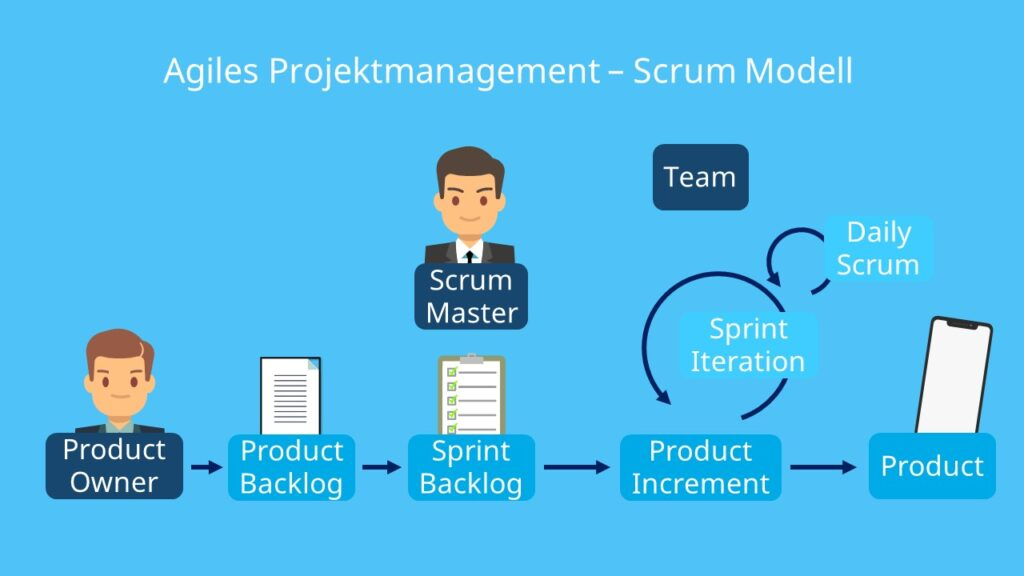
\includegraphics[width=0.9\textwidth]{pics/ScrumAblauf.jpg}
    \centering
    \caption{Veranschaulichung von Scrum https://studyflix.de/wirtschaft/scrum-methode-3426}
    \label{fig:scrum}
\end{figure}

\subsubsection{Product Backlog}
Der Product Backlog enthält sämtliche Anforderungen an das Produkt. Diese Anforderungen werden 
Schritt für Schritt in Sprints bearbeitet. In einem separaten Meeting wird dann entschieden, 
welche Anforderungen aus dem Product Backlog im jeweiligen Sprint abgearbeitet werden. Der Backlog
kann Qualitätsanforderungen, Funktionale Anforderungen, User Stories, Fehler (Bugs) und 
Verbesserungen enthalten. \cite{noauthor_scrum_nodate}

\subsubsection{Burn Down Chart}
Burn Down Charts visualisieren die Arbeit, die zum aktuellen Zeitpunkt noch zu erledigen ist. 
Es lässt sich anhand des Diagrammes die Arbeitsgeschwindigkeit des Teams ableiten.
Das Burn Down Chart eignet sich weiters dafür, die Interaktionen bzw. Sprints zu kontrollieren und 
wenn nötig kontrollierend eingreifen. \cite{noauthor_burn-down-chart_2021}, \cite{noauthor_was_nodate-4}

\subsubsection{GitHub-Tokens}
Persönliche Zugangs-Token (PATs) sind eine Alternative zur Verwendung von Passwörtern für die 
Authentifizierung bei GitHub. Als Sicherheitsvorkehrung entfernt GitHub automatisch persönliche 
Zugangstoken, die seit einem Jahr nicht mehr verwendet wurden. Seit Juli 2020 sind 
Authentifizierungstoken statt Passwörter zu verwenden. \cite{noauthor_token_2020}, \cite{noauthor_creating_nodate}

\section{Problemlösung}
\subsection{GitHub}
Die Wahl Git zur Versionskontrollierung und Kollaboration zu verwenden, ist aus offensichtlichen Gründen der einfachen 
Zusammenarbeit und Codezusammenführung getroffen worden. Für den Provider wurde sich für GitHub entschieden, da das Team 
viel Erfahrung im Umgang mit der Plattform besitzt und daher der Gebrauch naheliegend ist. In Abbildung (siehe Abb. \ref{fig:gituse}) wird die Verwendung 
von GitHub gezeigt. In Abbildung (siehe Abb. \ref{fig:gituse2}) wird die gemeinsame und parallele Arbeit dargestellt. 
Das Zusammenfügen des Quellcodes konnte hauptsächlich durch Git automatisch durchgeführt werden. Einige Zusammenfügungen mussten allerdings 
manuell abgewickelt werden. 

\begin{figure}[H]
    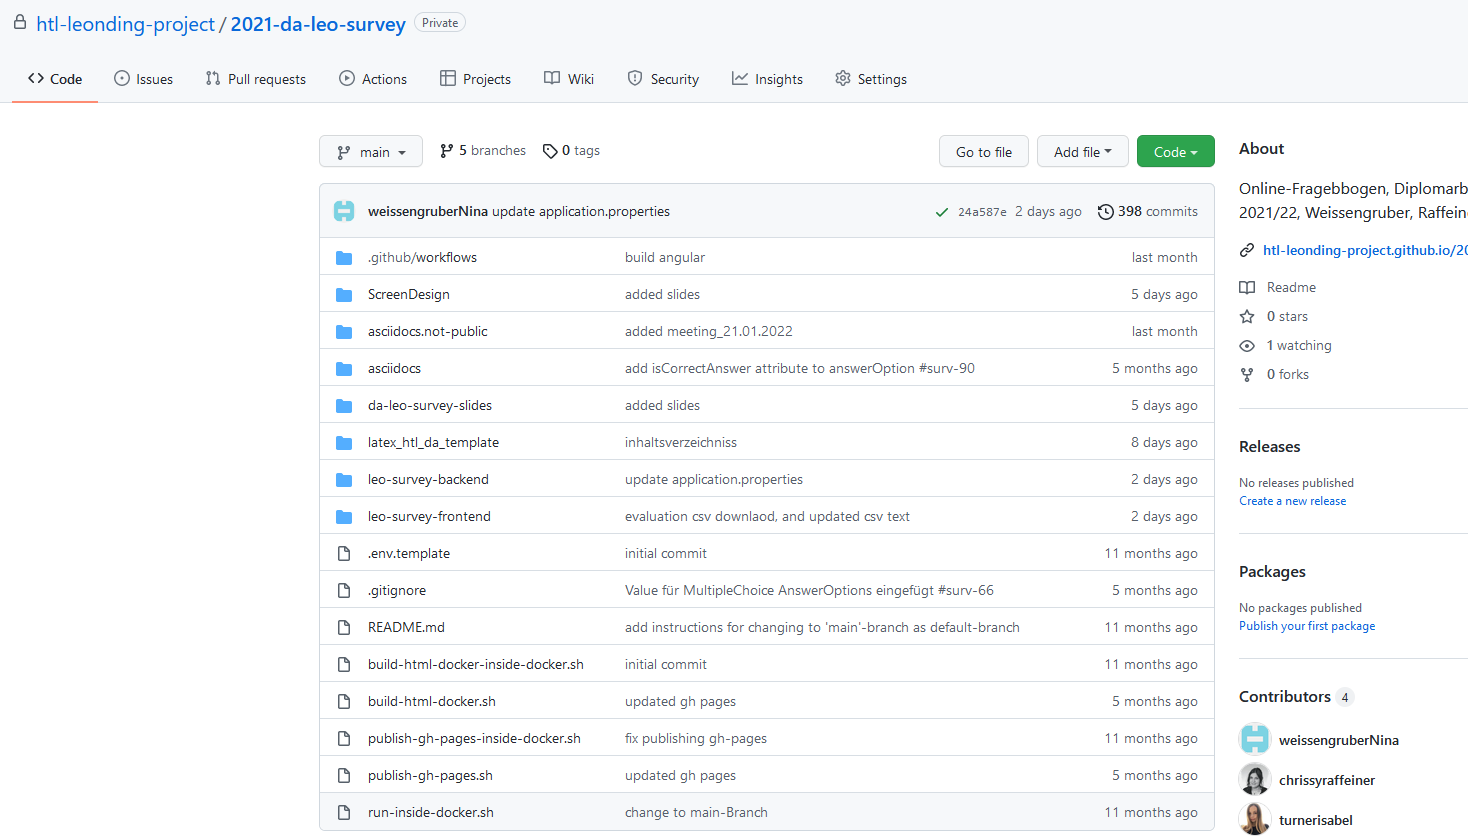
\includegraphics[width=1.0\textwidth]{pics/GitHub.PNG}
    \centering
    \caption{GitHub Repository von Leo-Survey}
    \label{fig:gituse}
\end{figure}

\begin{figure}[H]
    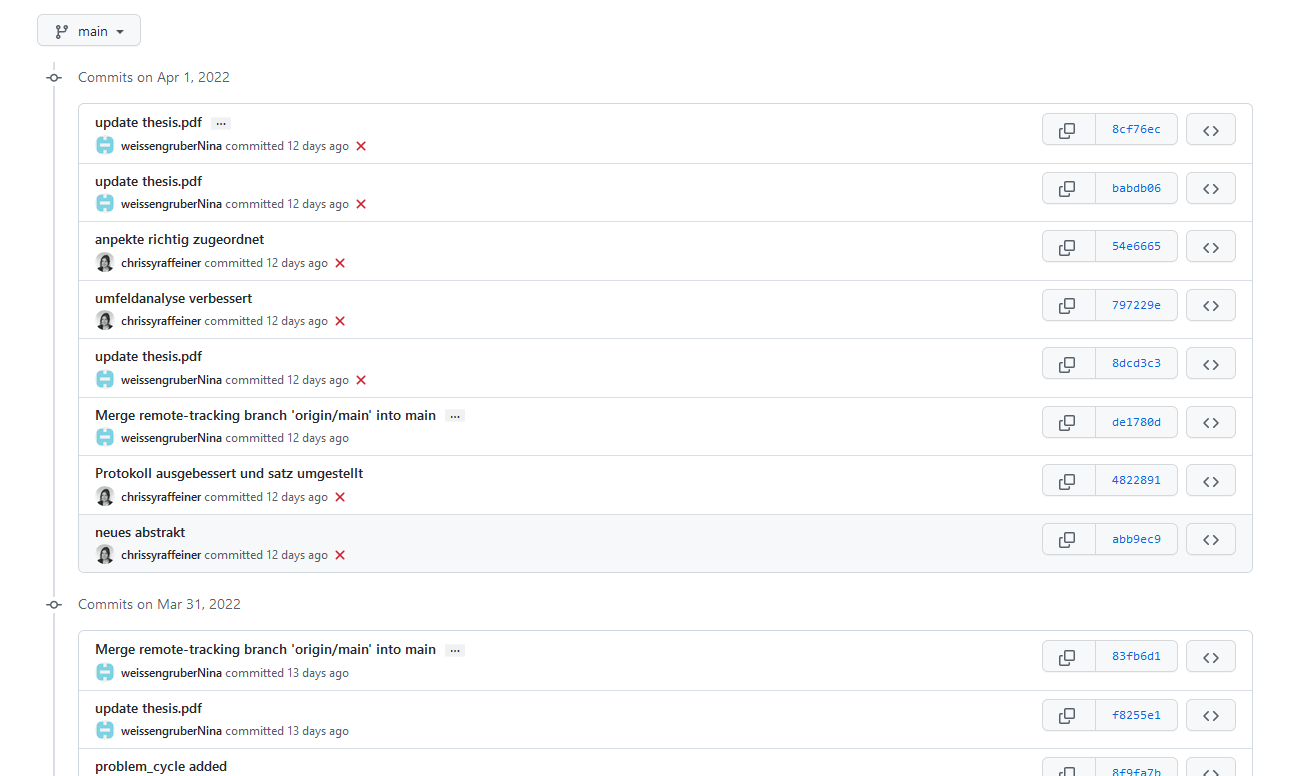
\includegraphics[width=1.0\textwidth]{pics/ComittHistory.PNG}
    \centering
    \caption{GitHub Repository von Leo-Survey Commites}
    \label{fig:gituse2}
\end{figure}

\subsection{GitDesktop}
Die Abbildung (siehe Abb. \ref{fig:git1}) zeigt die Verwendung von GitHub Desktop.
GitHub Desktop wurde hauptsächlich aus dem Grund verwendet, da zwei einzeln geöffnete Anwendungen (IntelliJ für das Backend) 
und (Visual Studio Code für das Frontend) die Änderungen des jeweils 
anderen Programmes nicht erkennen. Durch einen Neustart konnten die Änderungen dann erkannt werden. 
Da dies allerdings mit Aufwand verbunden ist wurde drauf verzichtet und 
GitHub Desktop verwendet. Die Anwendung löste dieses Problem.
\begin{figure}[H]
    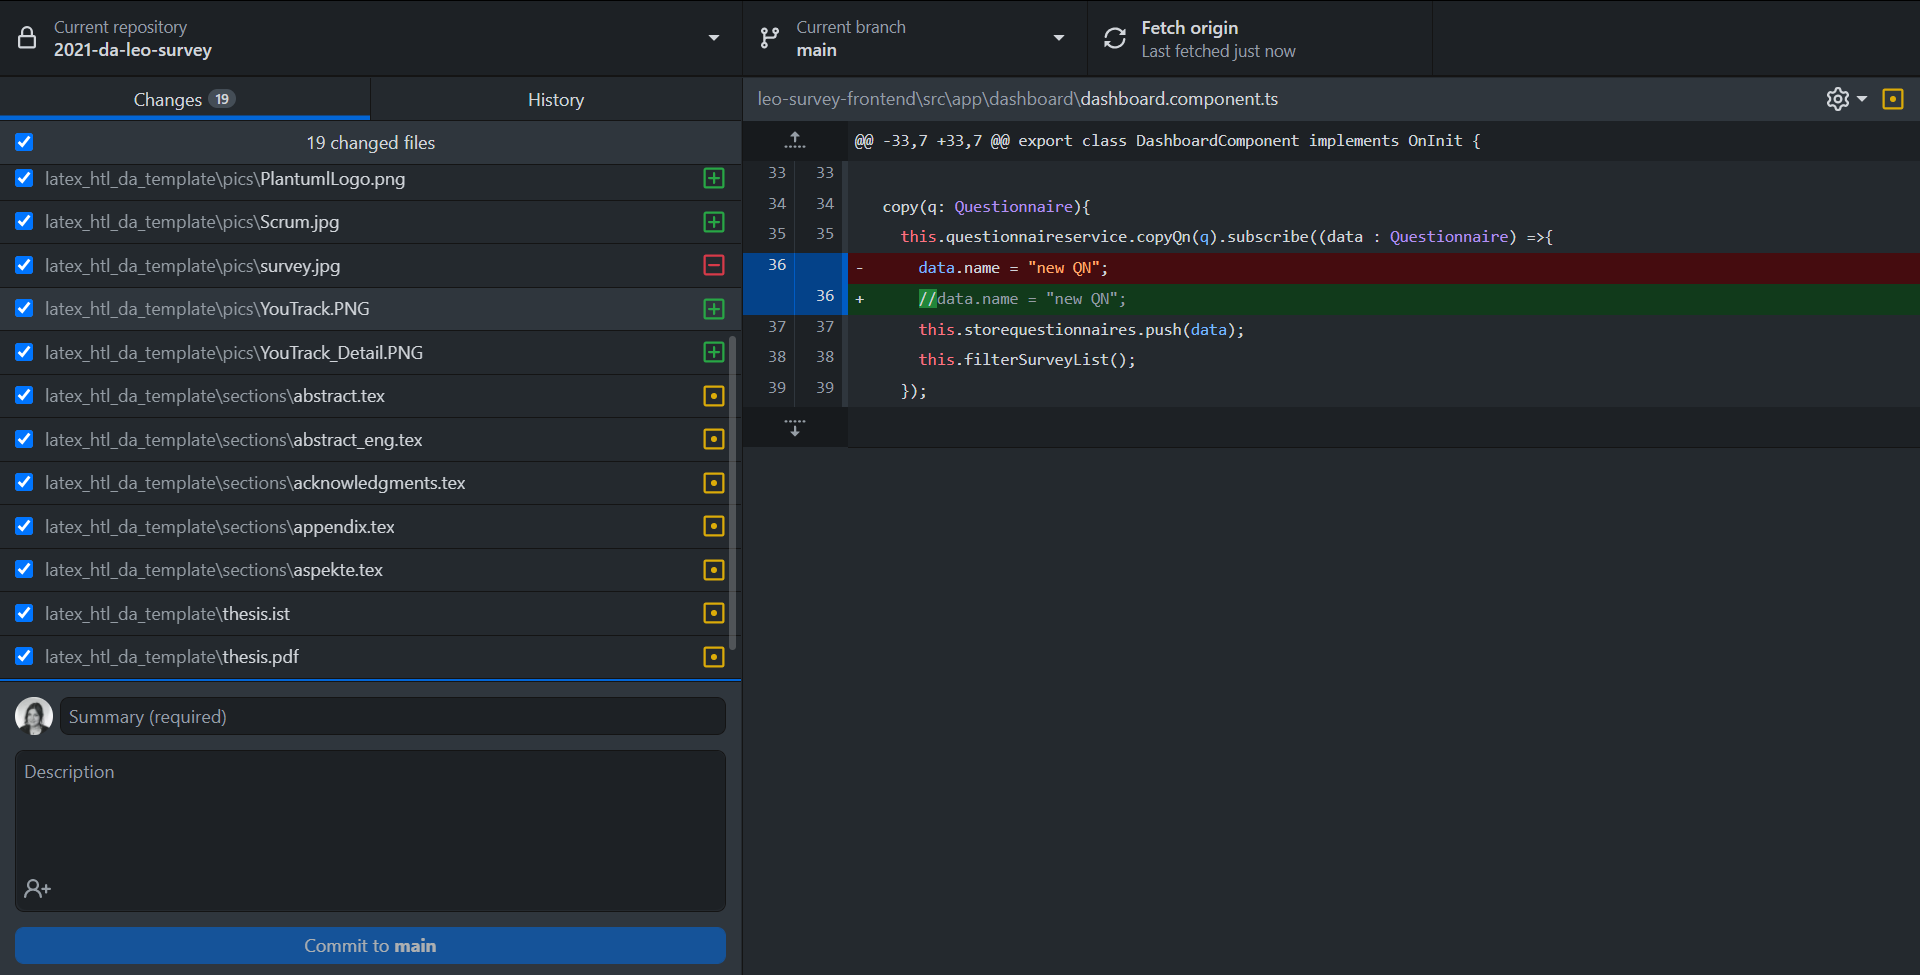
\includegraphics[width=1.0\textwidth]{pics/GitDesktop.PNG}
    \centering
    \caption{GitHub Desktop Beispiel}
    \label{fig:git1}
\end{figure}

\subsection{YouTrack}
Obwohl für das Projekt GitHub verwendet wurde, wurde sich gegen die Verwendung von GitHub Projektboards, Issues und Meilensteine
entschieden und für den Gebrauch von YouTrack. Hauptgrund dafür war, dass im Gegensatz zu GitHub, 
Tasks, Sprints etc. in YouTrack auf einer Seite übersichtlicher dargestellt werden konnten und auch 
zusätzliche Features wie das Burn Down Chart zu Verfügung stehen. Verbindet man YouTrack außerdem 
mit einem GitHub Repository verfügt man über die Funktion von automatisch einzuordnenden
Tasks. Die Projektboards wurden mit der YouTrack-Vorlage Kanban erstellt. 
Diese Vorlage erstellt automatisch 4 Schwimmbahnen (Open, In Progress, To Verify und Done). Die Vorlage kann bearbeitet werden. 
Es wurde allerdings auf eine Änderung verzichtet, da die Vorlage für die vorliegende Arbeit ausgereicht hat.

Die Abbildung (siehe Abb. \ref{fig:youtracksprint}) zeigt beispielhaft einen Sprint der Arbeit.
\subsection{GitHub-Anbindung in YouTrack}
\begin{figure}[H]
    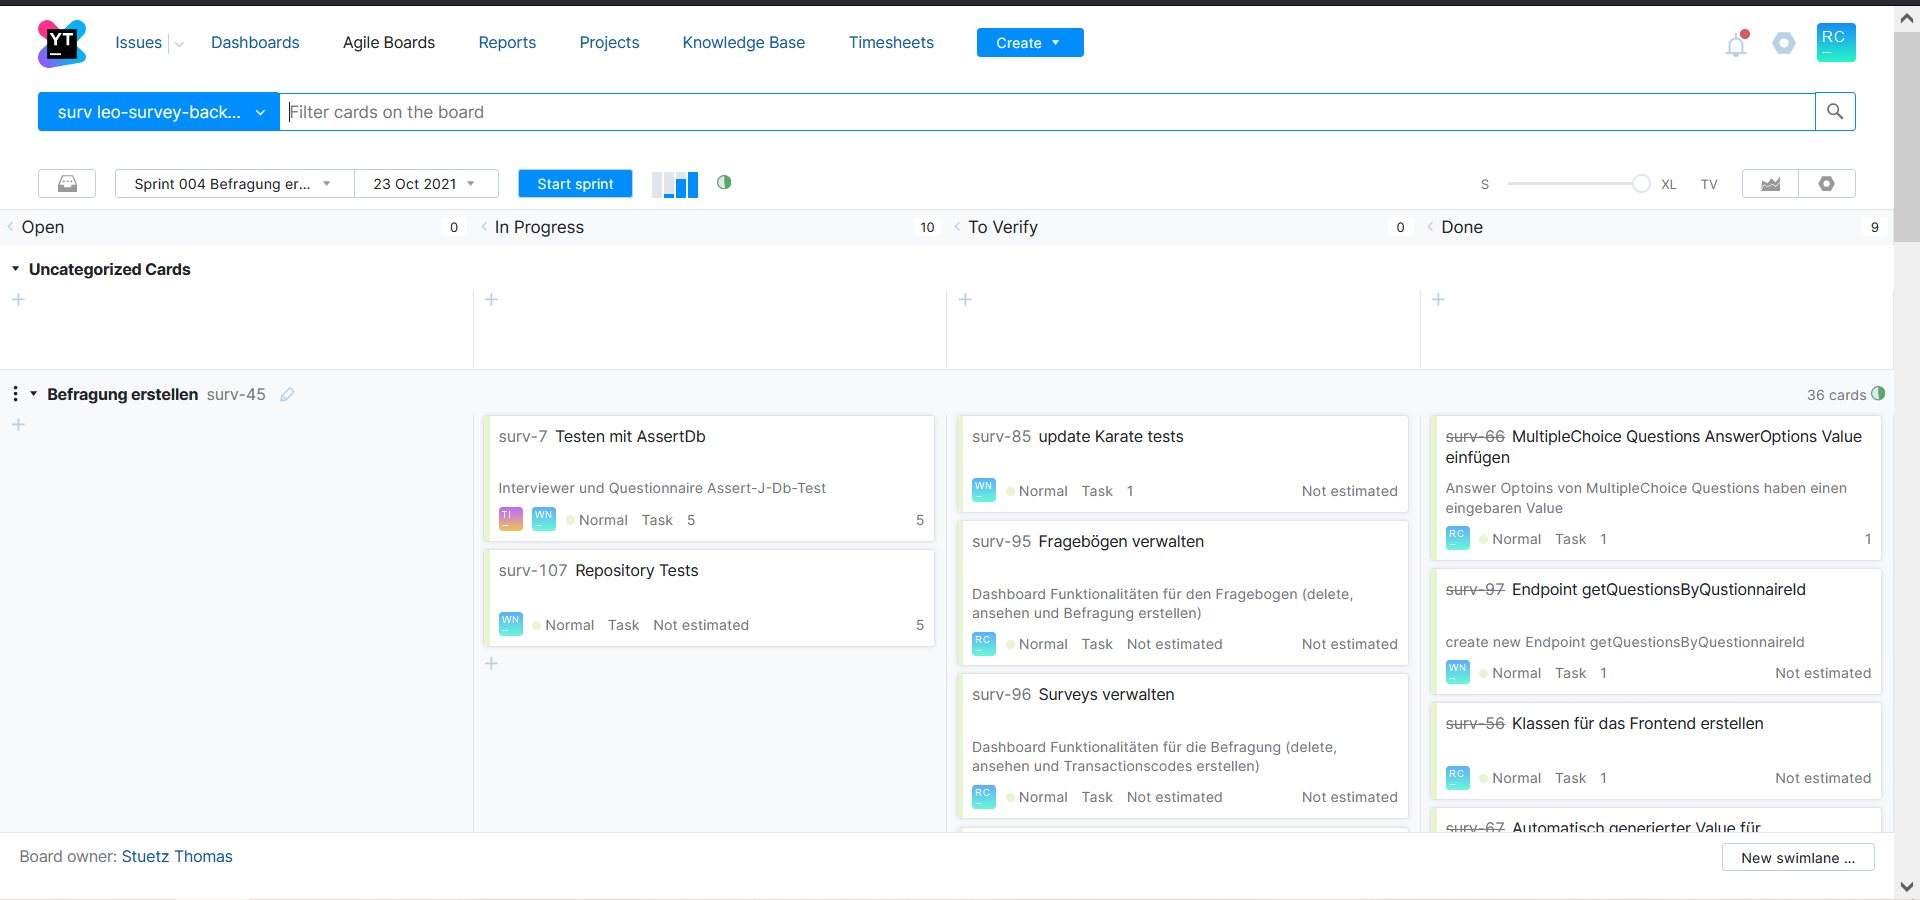
\includegraphics[width=1.0\textwidth]{pics/YouTrack.PNG}
    \centering
    \caption{YouTrack Sprint Beispiel}
    \label{fig:youtracksprint}
\end{figure}

Für designtechnische Aspekte, wie die Erstellung des Logos, Hintergrundbildes und ScreenDesigns wurde ein eigenes Projektboard 
erstellt. (siehe Abb. \ref{fig:youtracksprint2})  
\begin{figure}[H]
    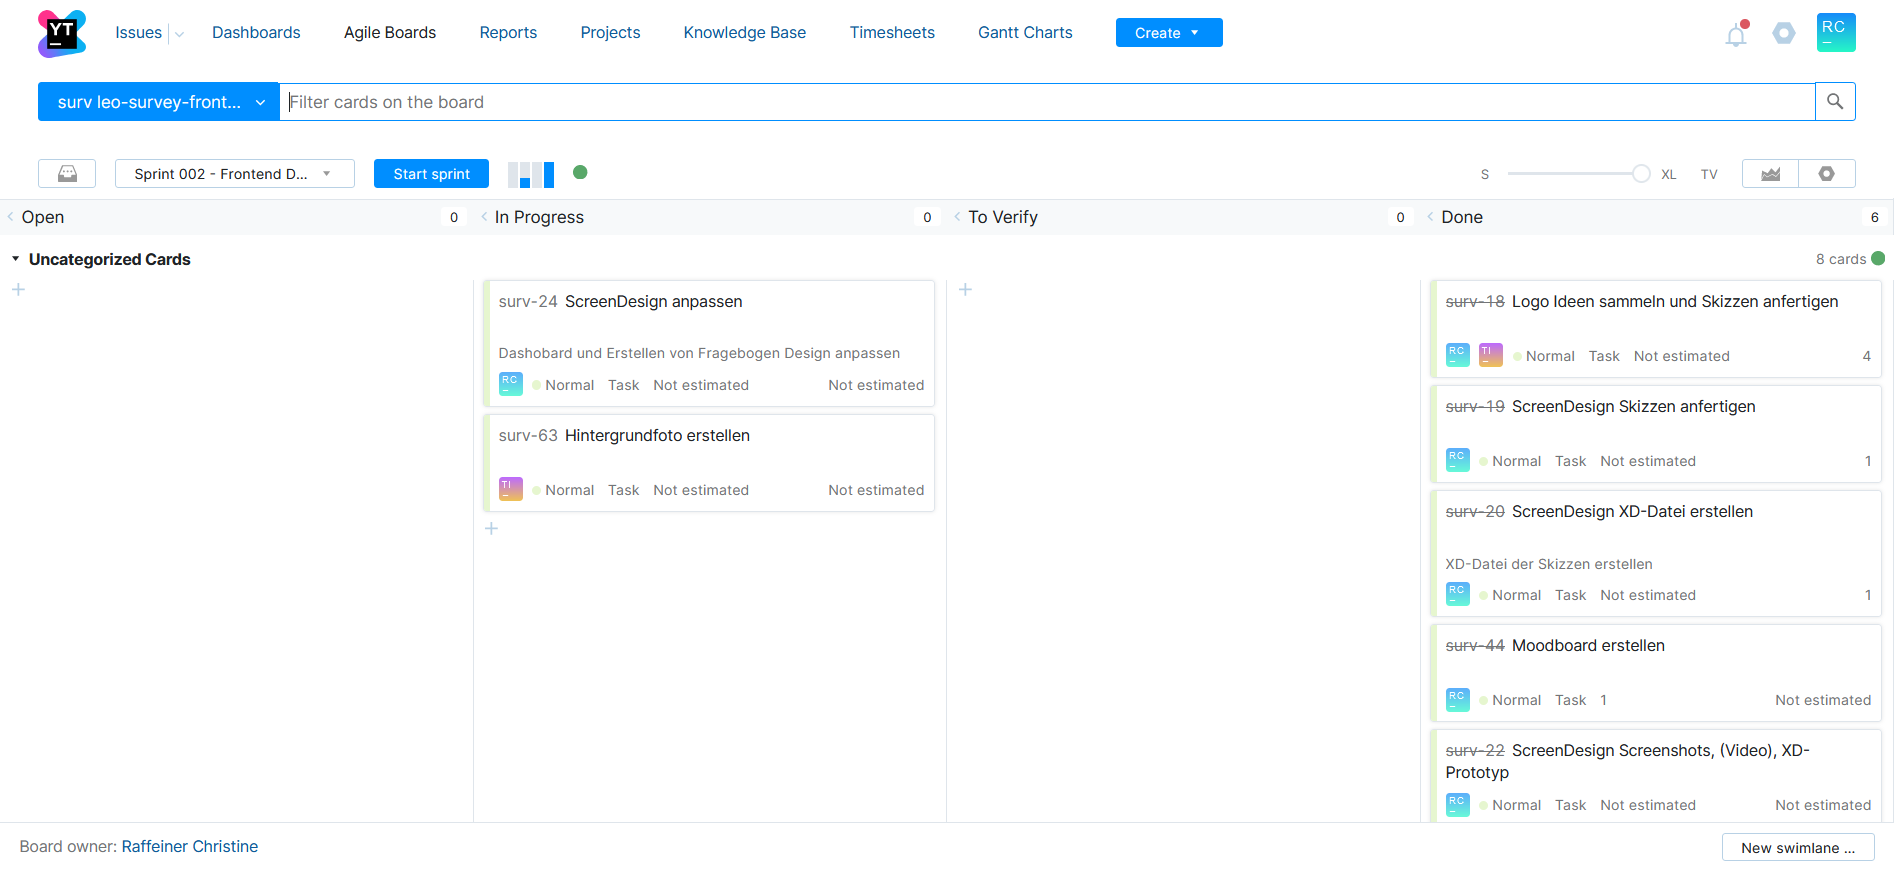
\includegraphics[width=1.0\textwidth]{pics/YouTrackfrontendboard.PNG}
    \centering
    \caption{GitHub-Anbindung in YouTrack}
    \label{fig:youtracksprint2}
\end{figure}

Abbildung (siehe Abb. \ref{fig:burndownchart}) zeigt beispielsweise ein Burn Down Chart aus der vorliegenden Arbeit.
Das Chart zeigt den Arbeitsaufwand des Deployments.  
Die grüne Line gibt den idealen Verlauf des noch zu tätigenden Arbeitsaufwandes an, sodass am Ende des Sprints alle Aufgaben erledigt sind.
Die blaue Line zeigt den tatsächlichen Verlauf des Arbeitsaufwandes und gibt Auskunft darüber, dass bis zum Ende des Sprints noch 
Arbeit zu erledigen ist. Zudem lässt sich daraus schlussfolgern, dass das Team die Vorgaben, bis zu diesem Zeitpunkt, 
eingehalten hat. (blaue Linie verläuft unter der grünen)
\begin{figure}[H]
    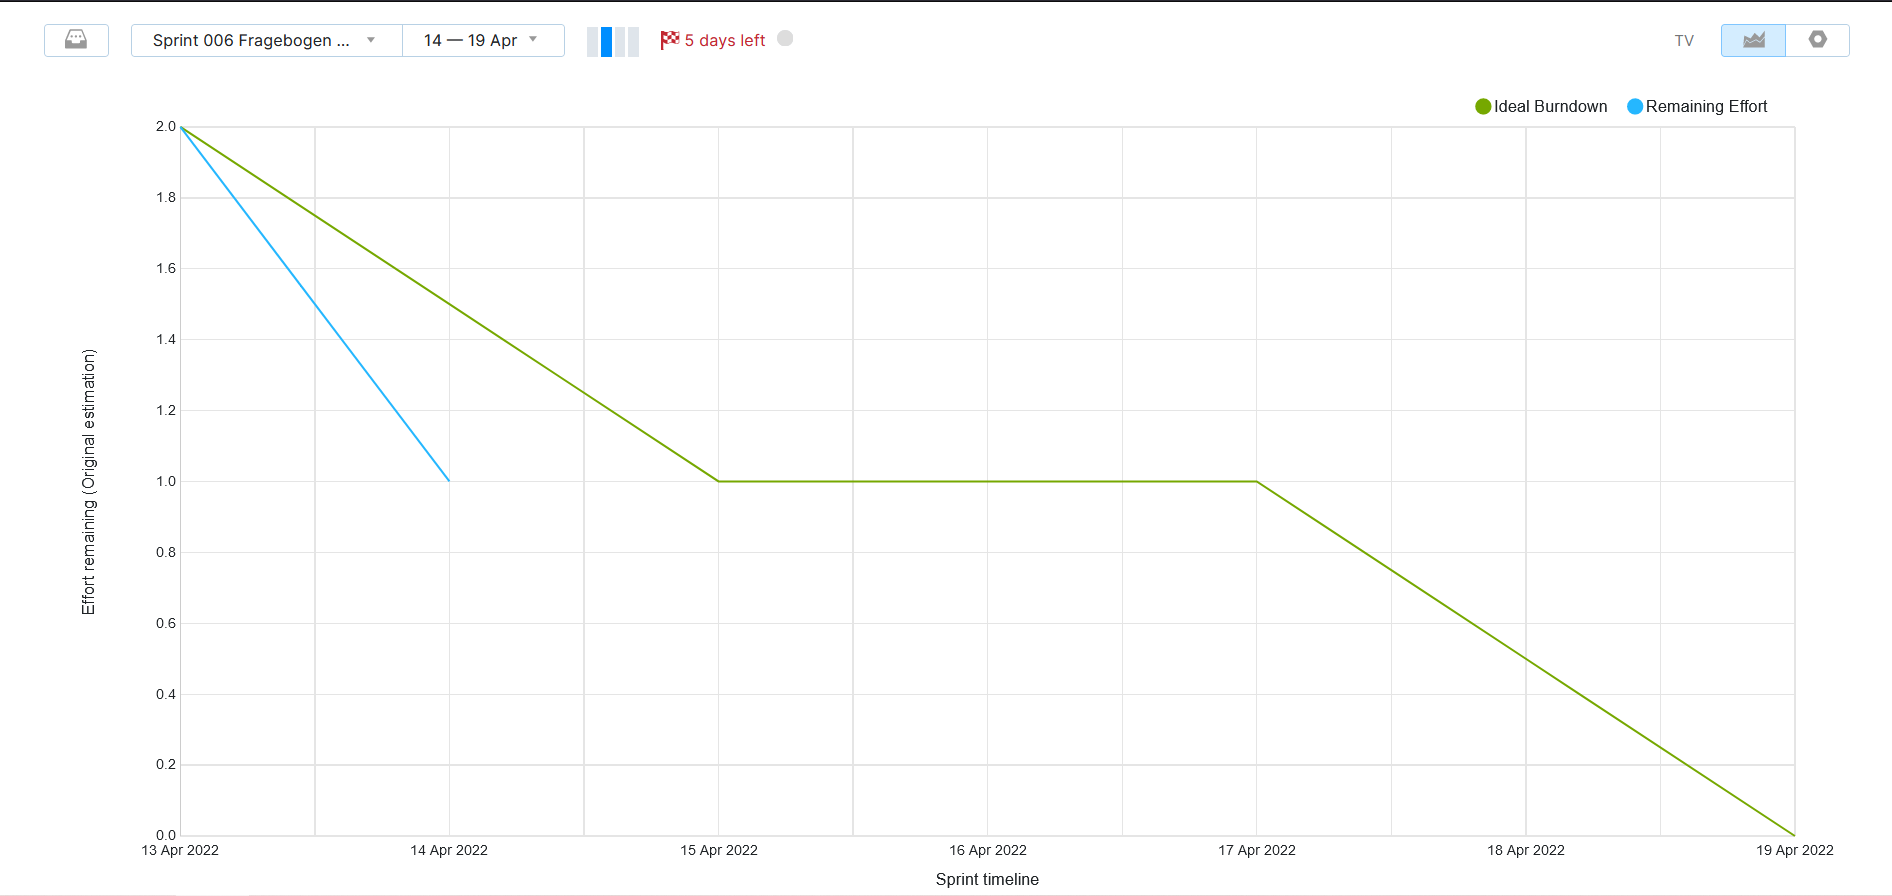
\includegraphics[width=1.0\textwidth]{pics/YouTrackBurnDownChart.PNG}
    \centering
    \caption{YouTrack Burn Down Chart Beispiel}
    \label{fig:burndownchart}
\end{figure}

Die Abbildung (siehe Abb. \ref{fig:youtrackGit}) zeigt die Anbindungen von YouTrack an das GitHub Repository, 
die dazu dient, beide Programme miteinander zu vereinen.
Wird ein Task in einer Commit-Message erwähnt, werden diese sonstigen Änderungen in der Detailansicht 
des Tasks angezeigt. Jeder angelegte Task bekommt eine Kennung in der Form \#surv-<zahl> (in diesem Beispiel
\#surv-7) und wird automatisch bei Erwähnung in einer Commit-Nachricht erkannt. Folgt auf die Kennung noch eine 
Bezeichnung einer Schwimmbahn wird der Task automatisiert in die angegebene 
Schwimmbahn geschoben (als Beispiel \#surv-7 To Verify). \cite{noauthor_youtrack_nodate}, \cite{noauthor_agile_nodate}
\begin{figure}[H]
    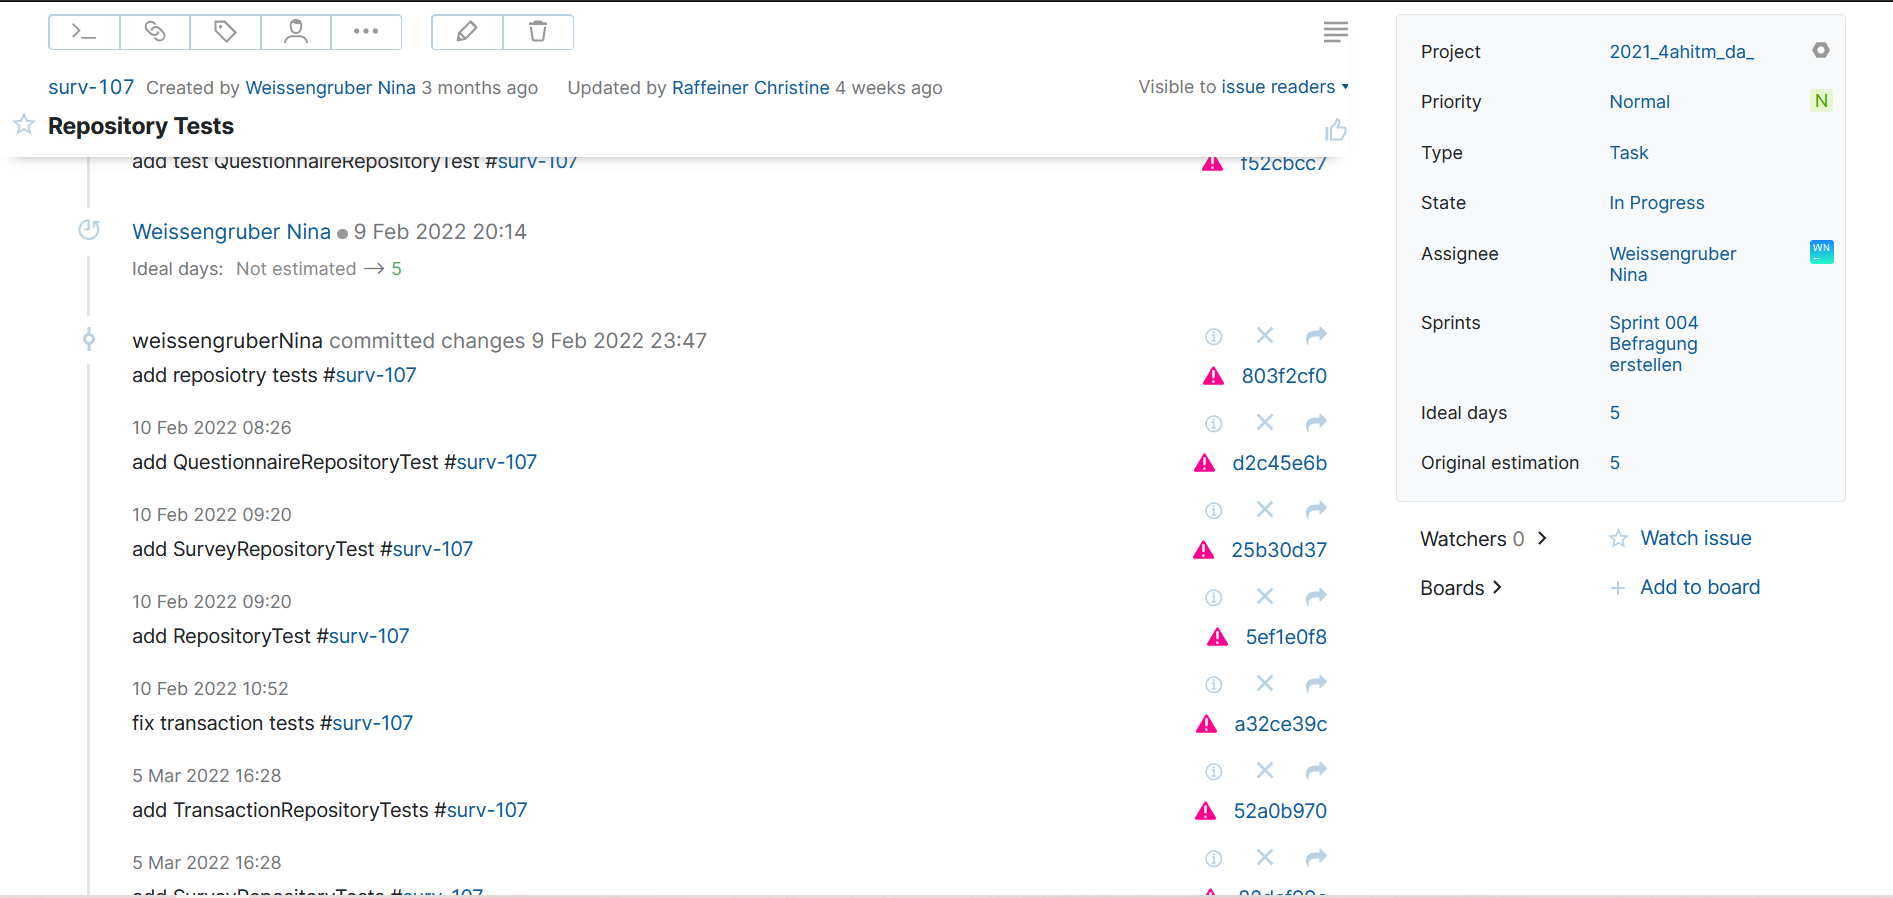
\includegraphics[width=1.0\textwidth]{pics/YoutrackGitCon.PNG}
    \centering
    \caption{GitHub-Anbindung in YouTrack}
    \label{fig:youtrackGit}
\end{figure}